\documentclass[tikz,border=8pt,multi=tikzpicture]{standalone}
\usepackage{amsmath}
\usepackage{xcolor}
\usetikzlibrary{arrows.meta, calc}

\definecolor{mainblue}{HTML}{001158}
\definecolor{accent}{HTML}{8592bc}
\definecolor{lightaccent}{HTML}{e7e9f2}

\tikzset{
  force/.style={-{Stealth[length=3mm]}, line width=1.2pt, color=mainblue},
  every node/.append style={font=\sffamily}
}

\begin{document}

% ---------- Concept sketch: concurrent force system ----------
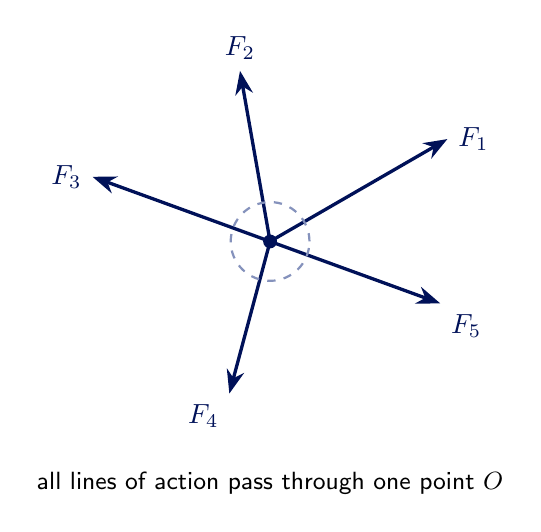
\begin{tikzpicture}
\coordinate (O) at (0,0);
\draw[force] (O) -- (30:2.6) node[right] {$F_1$};
\draw[force] (O) -- (100:2.2) node[above] {$F_2$};
\draw[force] (O) -- (160:2.4) node[left] {$F_3$};
\draw[force] (O) -- (255:2.0) node[below left] {$F_4$};
\draw[force] (O) -- (-20:2.3) node[below right] {$F_5$};
\draw[accent, dashed, line width=0.8pt] (0,0) circle (0.5);
\fill[mainblue] (O) circle (2.5pt);
\node[below=6pt] at (0,-2.6) {\small all lines of action pass through one point $O$};
\end{tikzpicture}

\end{document}
